\documentclass[dvipdfmx]{jsarticle}
\usepackage{tikz}
\usetikzlibrary{intersections, calc, arrows.meta}
\begin{document}
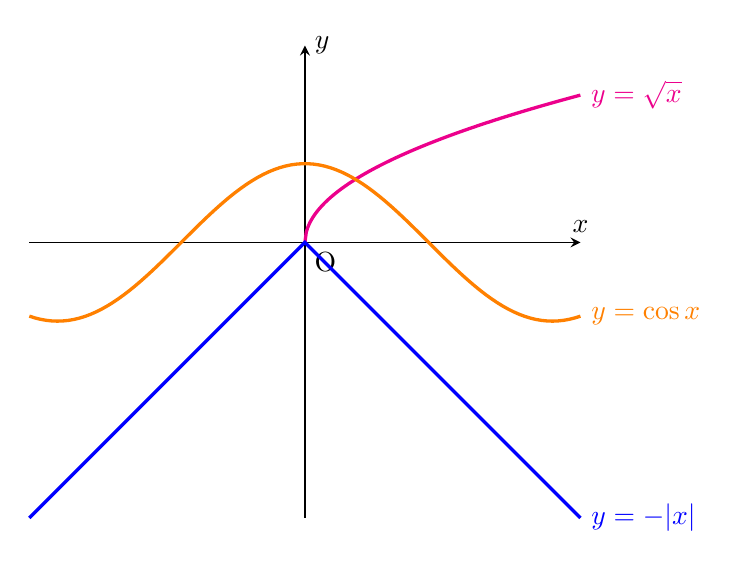
\begin{tikzpicture}
  \draw[->,>=stealth,semithick] (-3.5,0)--(3.5,0)node[above]{$x$}; %x軸
  \draw[->,>=stealth,semithick] (0,-3.5)--(0,2.5)node[right]{$y$}; %y軸
  \draw (0,0)node[below right]{O}; %原点
  \draw[magenta,very  thick,samples=200,domain=0:3.5] plot(\x,{sqrt(\x)})node[right]{$y=\sqrt{x}$};
  \draw[blue,very  thick,domain=-3.5:3.5] plot(\x,{-abs(\x)})node[right]{$y=-|x|$};
  \draw[orange,very  thick,samples=100,domain=-3.5:3.5] plot(\x,{cos(\x r)})node[right]{$y=\cos{x}$};
\end{tikzpicture}
\end{document}













